\chapter{General Introduction}
%\addstarredchapter{General Introduction}

\textbf{Macrosegregation} is a very known defect to metallurgical processes. Despite a great evolution achieved by active research during the last 60 years,
it remains partially understood. Macrosegregation is often  the consequence of several factors at the scale of a casting, all related to \emph{microsegregation} happening at the scale
of dendrites. Today, research in metallurgy focuses on a deeper understanding of such a connection between the different physical scales.
Solidification is not only a phase change, but also a complex transformation involving small scales like nucleation, medium scales
like grains growth and large scales like convection in the melt. From the nucleation theory to the mechanical behavior of metals, intricate phenomena combine to form defects in the final product. This has been seen in casting processes, such as continuous casting and ingot casting. Surface and volume porosity, hot tearing and composition heterogeneity are known defects to the casting community. After a brief introduction of these defects, macrosegregation will be the focus of this dissertation.

\section{Casting defects}
Undesired effects are inevitable in any industrial process. More importantly, a lot of defects in the casting industry can be disastrous in some situations where the cast product is not serviceable and hence rejected. This leads to a systematic product recycling, i.e. the product is ditched to be reheated, remelted and then cast again. From an economic point view, the operation is expensive timewise and profitwise. Understanding and preventing defects when possible, is thus crucial in the casting industry.
We focus hereafter on the main encountered defects.

\subsection*{Hot tearing} 
This defect, also denoted solidification cracking or hot cracking, occurs in the mushy zone at high solid fractions when a failure
or crack appears at specific locations, the hot spots. The temperature range in which the steel is vulnerable to hot tearing is known as the brittleness temperature range (BTR). It corresponds to solid fractions greater than \num{90}\%, with the liquid phase forming a discontinuous film. Many factors can cause the failure, but the main origin is a lack of liquid feeding required to compensate for the solidification shrinkage, in the presence of thermal stresses in the mushy region. Therefore, a crack initiates then propagates in the casting. 

\subsection*{Porosity}
%reference: \url{http://www.afsinc.org/about/content.cfm?ItemNumber=6933} \\
%reference: \url{http://en.wikipedia.org/wiki/Casting_defect} \\
Porosity is a void defect formed inside the casting or at the outer surface. It may attributed to two different factors.
Firstly, we speak of \emph{shrinkage porosity}, when a void forms as a result of density differences between the interdendritic liquid and solid
network, the latter being denser than the former. It is basically, the same reason that initiates hot cracks. 
The second factor is the presence of dissolved gaseous phases in the melt. According to \citet{dantzig_solidification_2009}, these gases may be initially in the melt, or created by the reaction between the metal and water found in the air or at trapped in grooves at the moulds surface. If the decreasing temperature and pressure drop in the liquid are large enough, the latter becomes supersaturated. Consequently, the nucleation of gaseous phase is triggered (just like when you open a cold bottle of coca-cola!).

\begin{figure}[h!] %h!
%Porosity1-2: http://www.afsinc.org/about/content.cfm?ItemNumber=6933
%Porosity3: http://www.weldreality.com/aluminumalloys.htm
%Porosity4: http://www.esab.com/global/en/education/new-lean-duplex-steels.cfm
\centering
   %------------
  \begin{subfigure}[t]{0.25\textwidth}
    \centering
	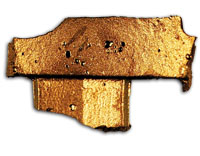
\includegraphics[width=\textwidth]{Chapter0/Graphics/porosity1.jpg}
	\caption{Gas porosity in casting}
    \label{fig:porosity1}
  \end{subfigure}
   %------------
   \hspace{2cm}
   \begin{subfigure}[t]{0.25\textwidth}
    \centering
	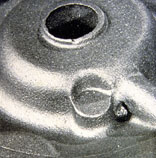
\includegraphics[width=\textwidth]{Chapter0/Graphics/porosity2.jpg}
	\caption{Shrinkage porosity}
    \label{fig:porosity2}
  \end{subfigure}
  %------------------------------
  \vskip\baselineskip
  %------------------------------
  \begin{subfigure}[t]{0.25\textwidth}
    \centering
	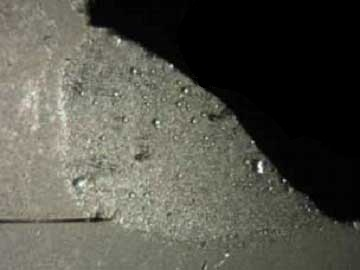
\includegraphics[width=\textwidth]{Chapter0/Graphics/porosity3.jpg}
	\caption{Gas porosity in aluminium welding}
    \label{fig:porosity3}
  \end{subfigure}
   %------------
  \hspace{2cm}
   \begin{subfigure}[t]{0.25\textwidth}
    \centering
	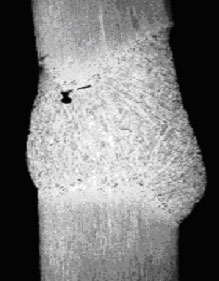
\includegraphics[width=\textwidth]{Chapter0/Graphics/porosity4.jpg}
	\caption{Xray of volume void inside welded duplex steel}
    \label{fig:porosity4}
  \end{subfigure}
   %------------
\caption{Examples of porosity in casting and welding} 
\label{fig:porosity}
\end{figure}

\subsection*{Freckles or segregated channels} 
The origin of this defect is microsegregation combined with gravity forces. They may appear 
in all casting processes, but are very specific to directional chill casting \citep{giamei_nature_1970}, mainly vertical chill casting.
Upon solidification, solid forms while rejecting some solute in the liquid due to partitioning (steels have a partition coefficient less than unity).
When the concentration of the liquid phase is high enough, a solutal or thermosolutal driving force is generated inside the mushy zone, transporting solute
by upward convection. Therefore "plume" shapes are often reported in the literature \citep{sarazin_studies_1992, schneider_modeling_1997}.
Segregation takes place at a medium scale (ranging from the scale of a few dendrites to a few hundreds of them), 
hence forms "long and narrow trails" as described by \citet{felicelli_simulation_1991}. Freckles are 
frequently formed by small equiaxed grains, probably caused by a uniform temperature gradient that settles as the channels become richer in solute. 
They can be observed on the ingot's surface, as well as in the volume.

\section{Macrosegregation}
Macrosegreation generally stems from a liquid flow transporting chemical species. Therefore, a non uniform composition could be observed on the scale 
of a casting, up to several meters in length. 
\section{Types}
\subsubsection*{Continuous casting}
\subsubsection*{Ingot casting}

\section{Causes}
Four main factors can (simultaneously) cause fluid flow leading to macrosegregation:
\subsubsection*{convection}
 Convection in the liquid can be driven by thermal and solutal gradients in the presence of gravity.
\subsubsection*{Movement of equiaxed grains} 
When thermal gradients are weak, or in the presence of inoculants, equiaxed grains can nucleate and grow in the liquid bulk. Being denser than the latter, they tend to fall
or move inside the liquid, transporting solute in their way.
\subsubsection*{Solidification shrinkage}
One may globally speak about \emph{shrinkage flow} caused by solidification shrinkage
and thermal contraction. The first type occurs in the mushy zone where the newly formed solid occupies a smaller volume than...
\subsubsection{Deformation of the solid} 
Compression and bulging are common in continous casting ....

\section{Industrial Worries}
\textbf{Steel production} has continuously increased over the years to meet the industrial needs. \autoref{fig:steel_production} shows this increase between 1980 and 2013 with a 
clear dominance of the Chinese production. Quality constraints have also increased where specific grades of steel are needed in critical applications such as mega-structures
in construction and  heavy machinery. Therefore, alloys with defects are considered vulnerable and should be avoided as much as possible during the casting process. As such, steelmakers have been investing
in research, with the aim of understanding better the phenomena leading to casting problems, and improve the processes when possible.

\begin{figure}[!h]
\centering
\begin{tikzpicture}
 \pgfkeys{%
    /pgf/number format/set thousands separator = {}}
\begin{axis}
[
	table/col sep=comma,
	smooth, %ybar
	stack plots=y,
	area style,
	enlarge x limits=false,
	legend pos=north west,
	scaled ticks=true,
	xlabel=Year,
	ylabel=Production (tons),
	xticklabel style={/pgf/number format/fixed},
	xtick={1980,1990,2000,2010},
	%x tick label style={rotate=45,anchor=east},
	%width=0.5\textwidth
]
\addplot table [x=Year, y expr=\thisrow{EU}*1000] {Chapter0/Data/steel_production.csv} \closedcycle ;
%\addlegendentry{EU (27)}
\addplot table [x=Year, y expr=\thisrow{China}*1000] {Chapter0/Data/steel_production.csv}\closedcycle;
%\addlegendentry{China}
\addplot table [x=Year, y expr=\thisrow{World}*1000] {Chapter0/Data/steel_production.csv}\closedcycle;
%\addlegendentry{World}
\legend{EU (27), China, World}
\end{axis}
%\addplot table [x expr=\coordindex, y=EU] {Chapter0/Data/steel_production.csv};
\end{tikzpicture}
\caption{Evolution curves of crude steel worldwide production from 1980 to 2013}
\label{fig:steel_production}
\end{figure}

\textbf{Simulation software} dedicated to alloy casting is one of the main research investments undertaken by steelmakers. These tools coming from academic research
are actively used to optimize the process. However, few are the tools that take into account the casting environment. For instance, the continuous casting process, in
\autoref{fig:cc_process}, is a chain process where the last steps involve rolls, water sprays and other components. A dedicated software is one that can provide the
geometric requirements with suitable meshing capabilities, as well as respond to metallurgical and mechanical requirements, mainly:
\begin{itemize}
\item handling moulds and their interaction with the alloy (thermal resistances ...)
\item handling alloy filling and predicting velocity in the liquid and mushy zone
\item handling thermomechanical stresses in the solid
\item handling multicomponent alloys and predicting macrosegregation
\item handling finite solute diffusion in solid phases
\item handling real alloy properties (not just constant thermophysical/thermomechanical properties)
\end{itemize}

\begin{figureth}
% textwidth 
{1.0}
%path 
{Chapter0/Graphics/cc_process}
% caption
{Main steps in a continuous casting plant}
% label
{cc_process}
\end{figureth}


\section{Objectives and outline}


\subsection*{\ccemlcc project}
Since its foundation in 1975, the European Space Agency (ESA) has been actively committed in the research field.
Their areas of activity cover not only exclusive space applications, but also fundamental science related to 
physics and other disciplines. This thesis takes part of the ESA project entitled \ccemlcc, abbreviating
"\textbf{C}hill \textbf{C}ooling for the \textbf{E}lectro-\textbf{M}agnetic \textbf{L}evitator in relation with 
\textbf{C}ontinuous \textbf{C}asting of steel".
The three-year contract from 2011 to 2014 denoted \ccemlcc II, was preceded by an initial project phase, \ccemlcc I,
from 2007 to 2010. The main focus is studying containerless solidification of steel under microgravity conditions. 
A chill plate is used to extract heat from the alloy, simulating the contact effect with a mould in continuous casting
or ingot casting.
CEMEF contributed to the work by proposing numerical models and simulation tools in view of predicting the chill cooling of steel droplets. 
A first model was developed by \citet{rivaux_simulation_2011} whereas the present discusses a new model. 
The experimental work considered various facilities and environments to set a droplet of molten alloy in levitation: electromagnetic levitation (EML) 
for ground-based experiments, microgravity in parabolic flight or sounding rockets and last, microgravity condition on-board the International Space Station (ISS)

\begin{figureth}
% textwidth 
{0.75}
%path 
{Chapter0/Graphics/eml1.jpg}
% caption
{Electromagnetic levitation}
% label
{eml}
\end{figureth}

\comment{in what ways does this project tries to alleviate the aforementionned problems ?
The two phases of CCEMLCC, together with the newly coming \ccemlcc III, aim to shape our understanding
of solidification with thermo-mechanical stresses under microgravity conditions.}


Numerical tools: Cimlib relying on PETSc, parallelized with MPICH2, paraview and python as tools for postprocess and analysis. \\
The previously mentionned simulation requirements are not met in a single casting software package. Nevertheless, \thercast is a promising tool that already 
handles a part of the above points. The current thesis developments are done using C++ language as a part of the
in-house code, known as \cimlib \citep{digonnet_cimlib:_2007, mesri_advanced_2009}. 
This fully parallel library is the main academic research support for \thercast.\\ \\ 

Aims of this research (+novelty of the work)\\ 
\begin{itemize}
\item solidification model with level set air-metal +darcy in the metal
\item Tracking of the interface induced by shrinkage
\end{itemize}
Each chapter content

\subsection*{Biblio test}
\citet{carozzani_direct_2013} is textual \\
\citep{carozzani_direct_2013} is parenthetical \\
%\section*{Trying \emph{SIUNITX}}
%Here i wana test the SI units package via the commands \num{.3e45} and the unit \si{\kilo\metre}
%then i wanted to see if we combine both via \SI{.3e45}{\kilo\metre} then finally my personal command
%\SI{231e-4}{\uacceleration} \\
%\SI{231e-4}{\ucomposition} C \\
%\SI{231e-4}{\uvelocity} \\
%\SI{231e-4}{\uconductivity} \\
%\SI{231e-4}{\umasscapacity} \\
%\SI{231e-4}{\uvolumecapacity} \\
%Will it work \num{.3e45}   ,  \num{3.45d-4}   , \numlist{10;30;50;70} ,  \numrange{10}{30}